\documentclass[letterpaper]{book}
\PassOptionsToPackage{usenames,dvipsnames,svgnames,table,xcdraw}{xcolor}
\PassOptionsToPackage{dvipsnames,svgnames,table,xcdraw}{enumitems}


%**************************************************************
%References for commands and symbols:
%1. https://en.wikibooks.org/wiki/LaTeX/Mathematics
%2. http://latex.wikia.com/wiki/List_of_LaTeX_symbols
%**************************************************************
\usepackage{scalerel}
\usepackage{setspace}

%\usepackage{url}
\usepackage{amsmath,amssymb}
\let\proof\relax 
\let\endproof\relax
\usepackage[cm]{fullpage}
%\usepackage{epsfig}
\usepackage{float}
\usepackage{alltt}
%\usepackage{psfrag,xr}
\usepackage[T1]{fontenc}
\usepackage{url}
\usepackage[utf8]{inputenc} % for boxes
\usepackage{pdfpages}
\usepackage{enumerate}
%\includepdfset{pagecommand=\thispagestyle{fancy}}
\usepackage{tcolorbox}

\usepackage{mathdots}
\usepackage{xfrac}
\usepackage{fix-cm} % Fixes warnings about missing fonts; see http://tex.stackexchange.com/questions/32378/xfrac-siunitx-gives-me-a-font-warning


% Font Settings
\usepackage{avant} % Use the Avantgarde font for headings
%\usepackage{mathptmx} % Use the Adobe Times Roman as the default text font together with math symbols from the Sym­bol, Chancery and Com­puter Modern fonts

\usepackage{subcaption}
%\usepackage{subfig}
\usepackage{graphicx} 
\graphicspath{{graphics/}}
%\usepackage[T1]{fontenc}
%\usepackage[usenames,dvipsnames,svgnames,table, xcdraw]{xcolor}
%\usepackage[caption=false,font=footnotesize]{subfig}
%\usepackage[utf8]{inputenc}
%\usepackage{bmpsize}
% \usepackage{caption}
% \captionsetup{size=footnotesize,
%     %justification=centering, %% not needed
%     skip=5pt, position = bottom}
% \let\proof\relax 
% \let\endproof\relax
%\usepackage{amsthm}
%\usepackage{algorithm}
\usepackage{algorithmicx}
%\usepackage{algpseudocode}
\usepackage{mathrsfs}
\usepackage[ruled,vlined]{algorithm2e}
\usepackage{times}
\usepackage{multicol}
%\usepackage[caption=false,font=footnotesize]{subfig}
\usepackage{amsfonts}
\usepackage[utf8]{inputenc}
\usepackage[T1]{fontenc}
\usepackage{textcomp}
\usepackage{balance}
%\usepackage[sort,numbers]{natbib}
\usepackage{multirow}
\usepackage{booktabs}
\usepackage{dblfloatfix} 

\usepackage{bbm}
\usepackage{bbold}
\usepackage{makecell}
\usepackage{hhline} % double-line in a table
% \usepackage[]{hyperref}
\usepackage[colorlinks]{hyperref}
\definecolor{BrickRed}{rgb}{0.7,0.15,0.15}
\hypersetup{
  colorlinks=true,pdfpagemode=UseNone,citecolor=black,linkcolor=black,urlcolor=BrickRed
}

\usepackage{comment}


\usepackage{xparse}
\usepackage{lipsum}
%\usepackage{subcaption}
\usepackage{soul} 
\usepackage{times}
%\usepackage{cite} % to group references
\usepackage[usenames,dvipsnames,svgnames,table,xcdraw]{xcolor}
% \usepackage[sort, numbers]{natbib}
%\usepackage{balance}
\usepackage{enumitem}

% \usepackage{hyperref}
% \usepackage{breakurl}[preserveurlmacro]


\usepackage{listings}
\usepackage{xcolor}
\lstset{literate=
  {á}{{\'a}}1 {é}{{\'e}}1 {í}{{\'i}}1 {ó}{{\'o}}1 {ú}{{\'u}}1
  {Á}{{\'A}}1 {É}{{\'E}}1 {Í}{{\'I}}1 {Ó}{{\'O}}1 {Ú}{{\'U}}1
  {à}{{\`a}}1 {è}{{\`e}}1 {ì}{{\`i}}1 {ò}{{\`o}}1 {ù}{{\`u}}1
  {À}{{\`A}}1 {È}{{\'E}}1 {Ì}{{\`I}}1 {Ò}{{\`O}}1 {Ù}{{\`U}}1
  {ä}{{\"a}}1 {ë}{{\"e}}1 {ï}{{\"i}}1 {ö}{{\"o}}1 {ü}{{\"u}}1
  {Ä}{{\"A}}1 {Ë}{{\"E}}1 {Ï}{{\"I}}1 {Ö}{{\"O}}1 {Ü}{{\"U}}1
  {â}{{\^a}}1 {ê}{{\^e}}1 {î}{{\^i}}1 {ô}{{\^o}}1 {û}{{\^u}}1
  {Â}{{\^A}}1 {Ê}{{\^E}}1 {Î}{{\^I}}1 {Ô}{{\^O}}1 {Û}{{\^U}}1
  {Ã}{{\~A}}1 {ã}{{\~a}}1 {Õ}{{\~O}}1 {õ}{{\~o}}1
  {œ}{{\oe}}1 {Œ}{{\OE}}1 {æ}{{\ae}}1 {Æ}{{\AE}}1 {ß}{{\ss}}1
  {ű}{{\H{u}}}1 {Ű}{{\H{U}}}1 {ő}{{\H{o}}}1 {Ő}{{\H{O}}}1
  {ç}{{\c c}}1 {Ç}{{\c C}}1 {ø}{{\o}}1 {å}{{\r a}}1 {Å}{{\r A}}1
  {€}{{\euro}}1 {£}{{\pounds}}1 {«}{{\guillemotleft}}1
  {»}{{\guillemotright}}1 {ñ}{{\~n}}1 {Ñ}{{\~N}}1 {¿}{{?`}}1
}
\definecolor{codegreen}{rgb}{0,0.6,0}
\definecolor{codegray}{rgb}{0.5,0.5,0.5}
\definecolor{codepurple}{rgb}{0.58,0,0.82}
\definecolor{backcolour}{rgb}{0.95,0.95,0.92}

\lstdefinestyle{mystyle}{
    backgroundcolor=\color{backcolour},   
    commentstyle=\color{codegreen},
    keywordstyle=\color{magenta},
    numberstyle=\tiny\color{black},
    stringstyle=\color{black},
    basicstyle=\ttfamily\normal,
    breakatwhitespace=false,         
    breaklines=true,                 
    captionpos=b,                    
    keepspaces=true,                 
    numbers=left,                    
    numbersep=5pt,                  
    showspaces=false,                
    showstringspaces=false,
    showtabs=false,                  
    tabsize=2
}
\lstset{style=mystyle}


\usepackage{mathtools}
\usepackage[english]{babel}
%\usepackage{minted}

\makeatletter
% \usepackage{tikz}
% \usetikzlibrary{calc}
% \newcommand*\circled[1]{\tikz[baseline=(char.base)]{
%     \node[shape=circle, draw, inner sep=1pt, 
%         minimum height={\f@size*1.6},] (char) {\vphantom{WAH1g}#1};}}
\makeatother

\newcommand{\rb}[1]{\raisebox{1.5ex}{#1}}
 \newcommand{\trace}{\mathrm{trace}}



%\def\real{\mathbb{R}}
\newcommand{\real}{\mathbb R}
\newcommand{\nat}{\mathbb N}   
\newcommand{\whole}{\mathbb Z}    
\newcommand{\cp}{\mathbb C}    
\newcommand{\rat}{\mathbb Q} 
\newcommand{\im}{\mathbb i}
\newcommand{\impart}[1]{\mathrm{imag} ( #1 )}
\newcommand{\repart}[1]{\mathrm{real} ( #1 )}
%\newcommand{\angle}[1]{\mathrm{angle} (#1 )}

%\def\real{\mathbb{R}}
\def\reals{\mathbb{R}} %????

\newcommand{\ds}{\displaystyle}
\newcommand{\mf}[2]{\frac{\ds #1}{\ds #2}}
\newcommand{\book}[2]{{Boyd, Page~#1, }{Prob.~#2}}
\newcommand{\Kuttler}[1]{Kuttler 2017, A First Course in Linear Algebra, Page(s)~#1}
\newcommand{\spanof}[1]{\mathrm{span} \{ #1 \}}
\newcommand{\colspanof}[1]{\mathrm{col~span} \{ #1 \}}
\newcommand{\nullspace}[0]{\mathrm{null}}
\newcommand{\nullity}[0]{\mathrm{nullity}}
\newcommand{\range}[0]{\mathrm{range}}
\newcommand{\cost}[0]{\mathrm{f}}
\newcommand{\rank}[0]{\mathrm{rank}}
\newcommand{\diag}[0]{\mathrm{diag}}

%%%%%%%%%%%%%%%%%%%
% Bruce added below
%%%%%%%%%%%%%%%%%%%
\newcommand{\transpose}{\mathsf{T}}
\DeclareDocumentCommand{\zeros}{ O{} }{\textbf{0}_{#1}}
\newcommand\inv[1]{#1\raisebox{1.15ex}{$\scriptscriptstyle-\!1$}}
\newcommand{\Exp}{\mathrm{Exp}}
\newcommand{\Log}{\mathrm{Log}}
\newtheorem{remark}{Remark}
%%%%%%%%%%%%%%%%%%%
% Bruce added above
%%%%%%%%%%%%%%%%%%%



%\newcommand{\dim}[0]{\mathrm{dim}}
 \newcommand{\cov}{\mathrm{cov}}
 \newcommand{\E}{\mathcal{E}}
\parindent 0pt

\newcommand{\notimplies}{%
  \mathrel{{\ooalign{\hidewidth$\not\phantom{=}$\hidewidth\cr$\implies$}}}}


\DeclareMathOperator*{\argmin}{arg\,min}
\DeclareMathOperator*{\argmax}{arg\,max}

\newcommand{\hilight}[1]{\colorbox{yellow}{#1}} % to use: \hl{this is some highlighted text}
\newcommand{\red}[1]{{\textcolor{red}{#1}}}
\newcommand{\blue}[1]{{\textcolor{blue}{#1}}}
\newcommand{\jwg}[1]{[{\textbf{\textcolor{red}{JWG: #1}}}]}
\newcommand{\mgj}[1]{[{\textbf{\textcolor{teal}{Maani: #1}}}]}
\newcommand{\bh}[1]{[{\textbf{\textcolor{blue}{Bruce: #1}}}]}


\newcommand\RED{\color{red}}
\newcommand\BLUE{\color{blue}}

\definecolor{note}{rgb}{0.3,0.7,0.25}
\definecolor{rephase}{rgb}{0.15,0.7,0.15}
\definecolor{bag}{rgb}{0.6,0.6,0.2}

 \newcommand\x{\times}
\newcommand\bigzero{\makebox(0,0){\text{\huge0}}}
\newcommand*{\bord}{\multicolumn{1}{c|}{}}
\newcommand*{\bordl}{\multicolumn{1}{|c}{}}

\newcommand*{\Qed}{\hfill $\blacksquare$}

\newcommand\doverline[1]{\ThisStyle{%
  \setbox0=\hbox{$\SavedStyle\overline{#1}$}%
  \ht0=\dimexpr\ht0-.15ex\relax% CHANGE .15 TO AFFECT SPACING
  \overline{\copy0}%
}}

\newcommand{\rob}{\textbb{ROB 101}}

% \newcommand*\circled[1]{\tikz[baseline=(char.base)]{
%     \node[shape=circle, draw, inner sep=1pt, 
%         minimum height={\f@size*1.6},] (char) {\vphantom{WAH1g}#1};}}
\makeatother







\usepackage{listings}
\usepackage{xcolor}

\definecolor{dkgreen}{rgb}{0,0.6,0}
\definecolor{gray}{rgb}{0.5,0.5,0.5}
\definecolor{mauve}{rgb}{0.58,0,0.82}
\definecolor{backcolour}{rgb}{0.98,0.92,0.97}
\definecolor{codegray}{rgb}{0.5,0.5,0.5}

%%
%% Julia definition (c) 2014 Jubobs
%%
\lstdefinelanguage{Julia}%
  {morekeywords={abstract,break,case,catch,const,continue,do,else,elseif,%
      end,export,false,for,function,immutable,import,importall,if,in,%
      macro,module,otherwise,quote,return,switch,true,try,type,typealias,%
      using,while},%
   sensitive=true,%
   alsoother={$},%
   morecomment=[l]\#,%
   morecomment=[n]{\#=}{=\#},%
   morestring=[s]{"""}{"""},%
   morestring=[m]{"}{"},%
}[keywords,comments,strings]%

\lstdefinestyle{mystyle}{
frame=tb,
  language=Julia,
  aboveskip=3mm,
  belowskip=3mm,
  showstringspaces=false,
  columns=flexible,
  basicstyle=\ttfamily,
  backgroundcolor=\color{backcolour},
  numberstyle=\tiny{\bf \color{black}},
  keywordstyle={\bf \color{blue}},
  commentstyle=\color{dkgreen},
  identifierstyle={\bf \color{black}},
  stringstyle=\color{mauve},
  breakatwhitespace=false,         
  breaklines=true,                 
  captionpos=b,                    
  keepspaces=true,                 
  numbers=left,                    
  numbersep=5pt,                  
  showspaces=false,                
  showstringspaces=false,
  showtabs=false,                  
  tabsize=2
}

\lstset{style=mystyle}

    % commentstyle=\itshape\color{purple!40!black},
    % identifierstyle=\color{blue},
    % backgroundcolor=\color{gray!10!white}
%\parindent

\makeatletter
\renewcommand{\frontmatter}{\cleardoublepage\@mainmatterfalse}
\renewcommand{\mainmatter}{\cleardoublepage\@mainmattertrue}
\makeatother

\title{Notes for Computational Linear Algebra\thanks{Inspired by Prof. Chad Jenkins}}
\date{}
\author{Jessy Grizzle\\ Robotics Institute, University of Michigan, Ann Arbor
\and Content contributed by Maani, Tribhi, Miley, Madhav, Kira, Michael, and Bruce}

%\doublespacing



\begin{document}
%\maketitle
\newtheorem{example}{Example}
\numberwithin{example}{chapter}



\begin{center}
    {\bf \Large Summary Chapters 1 through 7} \\
    Each Section is a Chapter in the Textbook
\end{center}

\setcounter{chapter}{1}
\setcounter{section}{-1}
\section{Tedium is a Good Motivator: A 3 x 3 Example}

Here is a \textit{system of linear equations} with variables $x_1, x_2, x_3$. 
\begin{equation}
\label{eq:SLE:Ex5}
\begin{aligned}
x_1+x_2+2x_3 &=7 \\
2x_1-x_2+x_3&=0.5\\
x_1 + 4 x_3 &=7
\end{aligned}
\end{equation}
The strategy for seeking a solution is the same as with two equations and two unknowns: solve for one of the variables in terms of the other variables, substitute into the remaining equations, simplify them, and repeat. We can start anywhere, so let's solve for $x_1$ in the bottom equation and plug that back into the two equations above it. Doing so gives us,
\begin{equation}
\label{eq:SLE:Ex5b}
   x_1 = 7 - 4 x_3 
\end{equation}
and then 
\begin{align*}
\underbrace{( 7 - 4x_3)}_{x_1} +x_2+ 2x_3 =7 & \implies x_2  - 2 x_3 = 0 \\
\underbrace{2( 7 - 4x_3)}_{2 x_1}-x_2+x_3=0.5 & \implies -x_2 -7 x_3 = -13.5
\end{align*}
\begin{align}
\label{eq:SLE:Ex5c}
 x_2  - 2 x_3 = 0 &\implies x_2 = 2 x_3\\
 -x_2 -7 x_3 = -13.5 & \implies \underbrace{-(2 x_3)}_{-x_2}-7x_3 = -13.5 \nonumber \\
 & \implies - 9 x_3 = -13.5  \nonumber\\
 &\implies x_3 = 1.5 \nonumber
\end{align}
Plugging ``$x_3=1.5$'' into \eqref{eq:SLE:Ex5b} gives $$x_1=7-4\cdot (1.5)=7-6=1.$$ 
And then from \eqref{eq:SLE:Ex5b}, we have that
$$x_2 = 2 x_3 = 2 \cdot (1.5) = 3. $$
Hence, the solution is
\begin{equation}
    \begin{bmatrix} x_1 \\ x_2 \\ x_3 \end{bmatrix} = \left[\begin{array}{l}
1.0 \\ 3.0 \\ 1.5
\end{array}  \right].
\end{equation}

\setcounter{chapter}{2}
\setcounter{section}{-1}
\section{Modern Notation: Ax = b and the Determinant}

\begin{example}
\label{ex:ExpressMatrixForm03}
Express the System of Linear Equations in Matrix Form: 
\begin{equation}
\begin{aligned}
x_1+x_2+2x_3 &=7 \\
2x_1-x_2+x_3&=0.5\\
x_1 + 4 x_3 &=7
\end{aligned}
\end{equation}
\end{example}

\textbf{Solution:} Note that we treat ``any missing coefficients'' (as in the ``missing $x_2$'' in the third equation) as being zeros! This is super important to remember. 
\begin{equation}
\label{eq:Axeqb04}
\begin{aligned}
x_1+x_2+2x_3 &=7 \\
2x_1-x_2+x_3&=0.5\\
x_1 + 4 x_3 &=7
\end{aligned}
\iff \underbrace{\left[\begin{array}{rrr} 1 & 1 & 2\\
2 & -1 & 1 \\ 1 & \boxed{0} & 4\end{array}\right]}_{A} \underbrace{\left[\begin{array}{c} x_1\\ x_2 \\ x_3\end{array}\right]}_{x} =   \underbrace{\left[\begin{array}{c} 7\\ 0.5 \\ 7\end{array}\right]}_{b}
\end{equation}
\Qed

\begin{tcolorbox}[sharp corners, colback=green!30, colframe=green!80!blue, title=\textbf{Enough Facts about the Determinant to Get Us Going}]
\begin{enumerate}[label={Fact~}{\arabic*}]

    \item \label{item:determinantFact1} A square system of linear equations (i.e.,  $n$ equations and $n$ unknowns), 
    $Ax=b,$
    has a unique solution $x$ for any $n\times 1$ vector $b$ \textbf{if, and only if}, $\det(A) \neq 0.$
    
     \item When $\det(A)=0$, the set of linear equations $Ax=b$ may have either no solution or an infinite number of solutions. To determine which case applies (and to be clear, only one case can apply), depends on how ``$b$ is related to $A$'', which is another way of saying that we will have to address this later in the course. 

     
    \item The determinant of the $2 \times 2$ square matrix 
    $A=\left[\begin{array}{cc} a & b \\ c & d \end{array} \right]$ is
  $\det(A):= a d - bc.$
  
  \item \textbf{Later, we learn that $\det(A\cdot B) = \det(A) \cdot \det(B)$ and LU Factorization allow us to compute the determinant of any square matrix, no matter how large.}
 
 
\end{enumerate}

\end{tcolorbox}

\setcounter{chapter}{3}
\setcounter{section}{-1}
\section{Matrices with Special Structure are Awesome}

{\bf \large We learn two key tools that we will use throughout the course:
\begin{itemize}
    \item Forward Substitution
    \item Back Substitution, aka Backward Substitution
\end{itemize}
}

\vspace*{1cm}

The general form of a lower triangular system with a non-zero determinant is
\begin{equation}
    \begin{aligned}
         a_{11} x_1 &= b_1  ~~~(a_{11} \neq 0) \\
          a_{21} x_1 + a_{22} x_2 &=b_2 ~~~(a_{22} \neq 0)\\
     \vdots &= \vdots \\
          a_{n1} x_1 + a_{n2} x_2 + a_{n3} x_3+ \cdots +  a_{nn} x_n &=b_n ~~~(a_{nn} \neq 0)
    \end{aligned}
\end{equation}
and the solution proceeds from top to bottom, like this
\begin{equation}
    \begin{aligned}
         x_1 &= \frac{b_1}{a_{11}}  ~~~(a_{11} \neq 0) \\
           x_2 &= \frac{b_2- a_{21} x_1}{a_{22}} ~~~(a_{22} \neq 0)\\
     \vdots &= \vdots \\
          x_n &=\frac{b_n-a_{n1} x_1 - a_{n2} x_2 - \cdots  -a_{n,n-1} x_{n-1}}{a_{nn}}    ~~~(a_{nn} \neq 0).
    \end{aligned}
\end{equation}

The general form of an upper triangular system with a non-zero determinant is
\begin{equation}
\label{eq:GeneralUpperTriangular}
    \begin{aligned}
     a_{11} x_1 + a_{12} x_2 + a_{13} x_3+ \cdots +  a_{1n} x_n &=b_1 ~~~(a_{11} \neq 0)\\
     a_{22} x_2 + a_{23} x_3 + \cdots +  a_{2n} x_n &=b_2 ~~~(a_{22} \neq 0)\\
       a_{33} x_3 + \cdots +  a_{3n} x_n &=b_3 ~~~(a_{33} \neq 0)\\
     \vdots &= \vdots \\
%     a_{n-1,n-1} x_{n-1} +  a_{n-1,n} x_n &=b_{n-1} ~~~(a_{n-1,n-1} \neq 0)\\
     a_{nn} x_n &= b_n  ~~~(a_{nn} \neq 0),
    \end{aligned}
\end{equation}
and the solution proceeds from the \textbf{bottom} of \eqref{eq:GeneralUpperTriangular} to its \textbf{top}, like this,
% \begin{equation}
%     \begin{aligned}
%       x_1  &=\frac{b_1- a_{12} x_2 - \cdots -  a_{1n} x_n}{a_{11}} &(a_{11} \neq 0)\\
%      x_2 &= \frac{b_2-  a_{23} x_3 - \cdots -  a_{2n} x_n}{a_{22}} &(a_{22} \neq 0)\\
%     %   a_{33} x_3 + \cdots +  a_{3n} x_n &=b_3 ~~~(a_{33} \neq 0)\\
%   \vdots &= \vdots & \vdots~~~~~ \\
%       x_{n-1}  &= \frac{b_{n-1}- a_{n-1,n} x_n}{a_{n-1,n-1}}  &(a_{n-1,n-1} \neq 0)\\
%       x_n &= \frac{b_n}{a_{nn}}  &(a_{nn} \neq 0),
%     \end{aligned}
% \end{equation}
\begin{equation}
    \begin{aligned}
    x_n &= \frac{b_n}{a_{nn}}  &(a_{nn} \neq 0) \medskip \\
     x_{n-1}  &= \frac{b_{n-1}- a_{n-1,n} x_n}{a_{n-1,n-1}}  &(a_{n-1,n-1} \neq 0)\\
       \boldmath \vdots \unboldmath~~~ &=~~~~  \boldmath \vdots \unboldmath &  \boldmath \vdots \unboldmath~~~~~ \\
        x_2 &= \frac{b_2-  a_{23} x_3 - \cdots -  a_{2n} x_n}{a_{22}} &(a_{22} \neq 0)\\
      x_1  &=\frac{b_1- a_{12} x_2 - \cdots -  a_{1n} x_n}{a_{11}} &(a_{11} \neq 0)
    \end{aligned}
\end{equation}

\vspace*{1cm}


{\bf For those of you with a ``visual memory''}, here is a graphical representation for upper and lower triangular matrices
\begin{equation}
\text{(lower triangular)}
 \left[
    \begin{array}{ccccc}
  \x     & \bordl &       &  & \\ \cline{2-2}
\x       & \x    & \bordl  &\bigzero & \\ \cline{3-3}
 \x      & \x    & \x  & \bordl    & \\ \cline{4-4}
  \x      & \x    & \x  &  \x & \bordl  \\  \cline{5-5}
    \x    & \x       & \x    & \x    & \x 
  \end{array}\right] \hspace*{2cm}  
\left[
    \begin{array}{ccccc}
    \x    & \x       & \x    & \x    & \x \\ \cline{1-1}
    \bord & \x       & \x    & \x    & \x \\ \cline{2-2}
          & \bord    & \x    & \x    & \x \\ \cline{3-3}
          & \bigzero & \bord & \x    & \x \\ \cline{4-4}
          &          &       & \bord & \x \\ 
  \end{array}\right]  \text{(upper triangular).} 
\end{equation}
\textbf{ Lower:}  everything above the diagonal is zero. \textbf{Upper:} everything below the diagonal is zero. For us to be able to solve the equations for arbitrary values $b$ on the right-hand side of $Ax=b$, we need the elements on the diagonal to be non-zero.\\
\begin{equation}
\label{eq:GeneralUpperTriangular}
    \begin{aligned}
     a_{11} x_1 + a_{12} x_2 + a_{13} x_3+ \cdots +  a_{1n} x_n &=b_1 ~~~(a_{11} \neq 0)\\
     a_{22} x_2 + a_{23} x_3 + \cdots +  a_{2n} x_n &=b_2 ~~~(a_{22} \neq 0)\\
       a_{33} x_3 + \cdots +  a_{3n} x_n &=b_3 ~~~(a_{33} \neq 0)\\
     \vdots &= \vdots \\
%     a_{n-1,n-1} x_{n-1} +  a_{n-1,n} x_n &=b_{n-1} ~~~(a_{n-1,n-1} \neq 0)\\
     a_{nn} x_n &= b_n  ~~~(a_{nn} \neq 0),
    \end{aligned}
\end{equation}

\vspace*{1cm}

{\bf \Large Important Fact: } {\large The determinant of a square triangular matrix is the product of the terms on the diagonal}.\\

\newpage

\setcounter{chapter}{4}
\setcounter{section}{-1}
\section{Matrix Multiplication: Insight Can Come from Strange Places}

{\bf \large ``The Finger Tracing Method''} We partition the $n \times k$ matrix $A$ into rows and the  $k \times m$ matrix $B$ into columns, as in 
\begin{equation}
   A= \left[\begin{array}{cccc} a_{11}& a_{12}& \cdots & a_{1k} \medskip \\
 a_{21}& a_{22}& \cdots & a_{2k}  \\
 \vdots & \vdots&  \ddots & \vdots \\
 a_{n1}& a_{n2}& \cdots & a_{nk} 
 \end{array}\right] = 
\left[\begin{array}{c} a_1^{\rm row}\\
a_2^{\rm row} \\
\vdots \\
a_n^{\rm row}\end{array}\right]  = \left[\begin{array}{c}\boxed{a_{11}~~ a_{12}~~ \cdots~~ a_{1k}}  \medskip \\
\boxed{a_{21}~~ a_{22}~~ \cdots~~ a_{2k}} \\
\vdots \\
\boxed{a_{n1}~~ a_{n2}~~ \cdots~~ a_{nk}}\end{array}\right]
\end{equation}
and
\begin{equation}
   B= \left[\begin{array}{cccc} b_{11}& b_{12}& \cdots & b_{1m} \\
 b_{21}& b_{22}& \cdots & b_{2m}  \\
 \vdots & \vdots&  \ddots & \vdots \\
 b_{k1}& b_{k2}& \cdots & b_{km} 
 \end{array}\right] =
\left[\begin{array}{cccc} b_1^{\rm col} & b_2^{\rm col} & \cdots & b_m^{\rm col}\end{array}\right]  = \left[ \boxed{\begin{array}{c} b_{11} \\ b_{21}\\ \vdots \\ b_{k1}\end{array} }~~~
\boxed{\begin{array}{c} b_{12} \\ b_{22}\\ \vdots \\ b_{k2}\end{array} }~~~\cdots~~~
\boxed{\begin{array}{c} b_{1m} \\ b_{2m}\\ \vdots \\ b_{km}\end{array} }\right],
\end{equation}
then
\begin{equation}
   A \cdot B:= 
\left[\begin{array}{cccc}  a_1^{\rm row} \cdot b_1^{\rm col} & a_1^{\rm row} \cdot b_2^{\rm col} & \cdots & a_1^{\rm row} \cdot b_m^{\rm col} \medskip  \\
a_2^{\rm row} \cdot b_1^{\rm col} & a_2^{\rm row} \cdot b_2^{\rm col} & \cdots & a_2^{\rm row} \cdot b_m^{\rm col} \\
\vdots & \vdots & \ddots & \vdots \\
a_n^{\rm row} \cdot b_1^{\rm col} & a_n^{\rm row} \cdot b_2^{\rm col} & \cdots & a_n^{\rm row} \cdot b_m^{\rm col}
\end{array}\right].
\end{equation}
Another way to see the pattern is like this
\begin{equation}
\label{eq:RowColumnMatrixMultiplication}
   A \cdot B:=  \left[\begin{array}{c}\boxed{a_{11}~~ a_{12}~~ \cdots~~ a_{1k}}  \medskip \\
\boxed{a_{21}~~ a_{22}~~ \cdots~~ a_{2k}} \\
\vdots \\
\boxed{a_{n1}~~ a_{n2}~~ \cdots~~ a_{nk}}\end{array}\right] \cdot 
\left[ \boxed{\begin{array}{c} b_{11} \\ b_{21}\\ \vdots \\ b_{k1}\end{array} }~~~
\boxed{\begin{array}{c} b_{12} \\ b_{22}\\ \vdots \\ b_{k2}\end{array} }~~~\cdots~~~
\boxed{\begin{array}{c} b_{1m} \\ b_{2m}\\ \vdots \\ b_{km}\end{array} }\right] =
%
\left[\begin{array}{cccc}  \sum\limits_{i=1}^k a_{1i}b_{i1} & \sum\limits_{i=1}^k a_{1i}b_{i2} & \cdots & \sum\limits_{i=1}^k a_{1i}b_{im}  \medskip \\
 \sum\limits_{i=1}^k a_{2i}b_{i1} & \sum\limits_{i=1}^k a_{2i}b_{i2} & \cdots & \sum\limits_{i=1}^k a_{2i}b_{im} \\
\vdots & \vdots & \ddots & \vdots \\
 \sum\limits_{i=1}^k a_{ni}b_{i1} & \sum\limits_{i=1}^k a_{ni}b_{i2} & \cdots & \sum\limits_{i=1}^k a_{ni}b_{im} \\
\end{array}\right].
\end{equation}

\begin{tcolorbox}[title=\textbf{Bottom Line on Standard Multiplication}] In the standard way of defining matrix multiplication, the
 $ij$-entry of $A \cdot B$ is obtained by multiplying the $i$-th row of $A$ by the $j$-th column of $B$ (whenever the multiplication makes sense, meaning that the number of columns of $A$ equals the number of rows of $B$). We will not use the following notation on a regular basis, but some of you make like it; if we let $[A \cdot B]_{ij}$ denote the $ij$-element of the matrix, $A\cdot B$, then 
 $$\textcolor{red}{\bf [A \cdot B]_{ij} := a_i^{\rm row} \cdot b_j^{\rm col}.} $$
\end{tcolorbox}
 
\newpage

{\bf \large ``Multiplication by Summing over Columns and Rows''} 

\begin{equation}
\begin{aligned}
   A \cdot B:=&  \left[\begin{array}{c}\boxed{a_{11}~~ a_{12}~~ \cdots~~ a_{1k}}  \medskip \\
\boxed{a_{21}~~ a_{22}~~ \cdots~~ a_{2k}} \\
\vdots \\
\boxed{a_{n1}~~ a_{n2}~~ \cdots~~ a_{nk}}\end{array}\right] \cdot 
\left[ \boxed{\begin{array}{c} b_{11} \\ b_{21}\\ \vdots \\ b_{k1}\end{array} }~~~
\boxed{\begin{array}{c} b_{12} \\ b_{22}\\ \vdots \\ b_{k2}\end{array} }~~~\cdots~~~
\boxed{\begin{array}{c} b_{1m} \\ b_{2m}\\ \vdots \\ b_{km}\end{array} }\right] \\
=&
%
\left[\begin{array}{cccc}  \sum\limits_{i=1}^k a_{1i}b_{i1} & \sum\limits_{i=1}^k a_{1i}b_{i2} & \cdots & \sum\limits_{i=1}^k a_{1i}b_{im}  \medskip \\
 \sum\limits_{i=1}^k a_{2i}b_{i1} & \sum\limits_{i=1}^k a_{2i}b_{i2} & \cdots & \sum\limits_{i=1}^k a_{2i}b_{im} \\
\vdots & \vdots & \ddots & \vdots \\
 \sum\limits_{i=1}^k a_{ni}b_{i1} & \sum\limits_{i=1}^k a_{ni}b_{i2} & \cdots & \sum\limits_{i=1}^k a_{ni}b_{im} \\
\end{array}\right] \text{ (we pull the sum outside the matrix)}\\
=& \sum\limits_{i=1}^k
\left[\begin{array}{cccc}   a_{1i}b_{i1} &a_{1i}b_{i2} & \cdots &  a_{1i}b_{im}  \medskip \\
     a_{2i}b_{i1} & a_{2i}b_{i2} & \cdots &  a_{2i}b_{im} \\
\vdots & \vdots & \ddots & \vdots \\
  a_{ni}b_{i1} & a_{ni}b_{i2} & \cdots &  a_{ni}b_{im} \\
\end{array}\right] \text{(we recognize what this is)}\\
=& \sum_{i=1}^{k} a_i^{\rm col} \cdot b_i^{\rm row} \\
=&
\left[ \boxed{\begin{array}{c} a_{11} \\ a_{21}\\ \vdots \\ a_{n1}\end{array} }~~~
\boxed{\begin{array}{c} a_{12} \\ a_{22}\\ \vdots \\ a_{n2}\end{array} }~~~\cdots~~~
\boxed{\begin{array}{c} a_{1k} \\ a_{2k}\\ \vdots \\ a_{nk}\end{array} }\right] \cdot  \left[\begin{array}{c}\boxed{b_{11}~~ b_{12}~~ \cdots~~ b_{1m}}  \medskip \\
\boxed{b_{21}~~ b_{22}~~ \cdots~~ b_{2m}} \\
\vdots \\
\boxed{b_{k1}~~ b_{k2}~~ \cdots~~ b_{km}}\end{array}\right]. \
\end{aligned}
\end{equation}

\vspace*{1cm}
{\bf \Large Important Fact: Order Matters} {\large In general $\boxed{A\cdot B \neq B \cdot A$}}.

\vspace*{1cm}
{\bf \Large Re-arranging Rows of an Equation Can be Helpful: Permutaion Matrices}

For example, suppose we want to do the following rearrangement
\begin{equation}
\label{eq:Permuation}
     \left[\begin{array}{r} 1 \\2 \\3 \\ 4 \\ 5\end{array} \right] \leftrightarrow \left[\begin{array}{r} 4 \\2 \\5 \\ 1 \\ 3\end{array} \right],
\end{equation}
where rows one and four are swapped and three and five are swapped. We have shown the arrow as going back and forth ($\leftrightarrow$) because applying the swap twice results in the original arrangement. To see the resulting structure at a matrix level, we put the $5 \times 5$ identity matrix on the left and the permutation matrix $P$ on the right
$$
I_5=\begin{bmatrix}
1&0&0&0&0\\
0&1&0&0&0\\
0&0&1&0&0\\
0&0&0&1&0\\
0&0&0&0&1
\end{bmatrix} \leftrightarrow
P=\begin{bmatrix}
0&0&0&1&0\\
0&1&0&0&0\\
0&0&0&0&1\\
1&0&0&0&0\\
0&0&1&0&0
\end{bmatrix}
$$
so that it is apparent that $P$ is just a re-ordering of the rows of $I$.


\begin{tcolorbox}[title=\textbf{Permutation Matrices, the Full Story}]
In general, matrices that consist of all ones and zeros, with each row and column having a single one, are called \textbf{permutation matrices}. \\

Later, we learned the matrix transpose, $P^\top$ and that $ P^\top \cdot P= P \cdot P^\top = I_n$.\\

Later, for permutation matrices,  we learned that $P^{-1} = P^\top$. 
\end{tcolorbox}


\setcounter{chapter}{5}
\setcounter{section}{-1}
\section{Banned Knowledge for Y1-Undergrads: Matrix Factorization: $P \cdot A = L \cdot U$}

\begin{center}

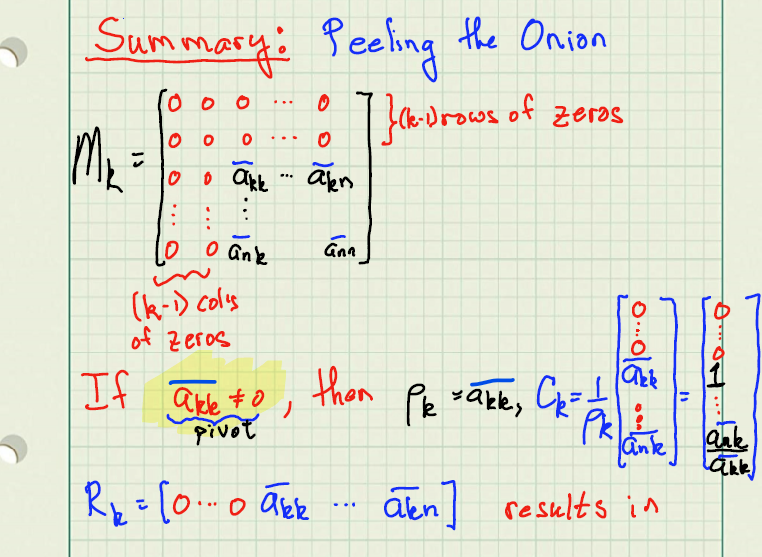
\includegraphics[width=0.9\columnwidth]{graphics/Summary/PeelingTheOnionPart01.png}

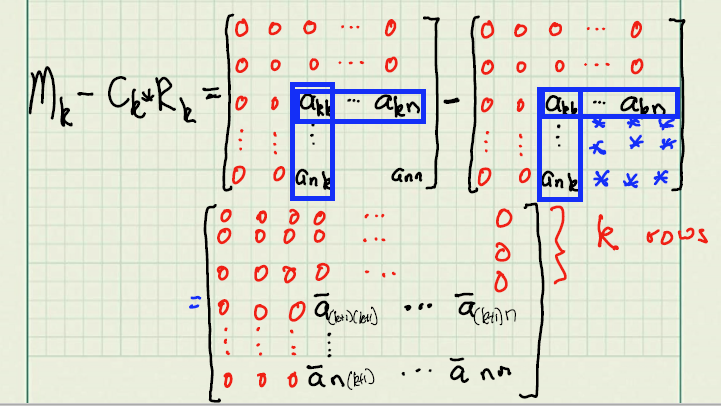
\includegraphics[width=0.9\columnwidth]{graphics/Summary/PeelingTheOnionPart02.png}

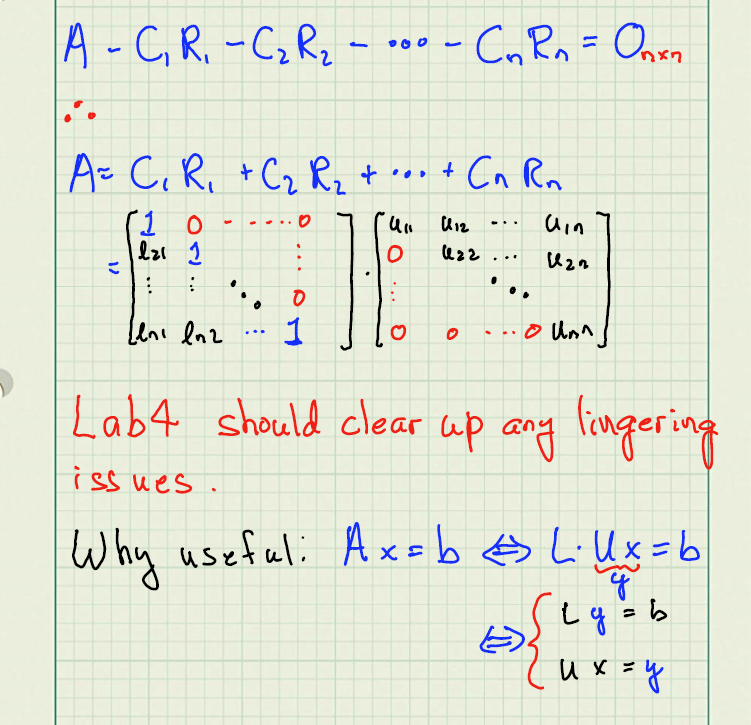
\includegraphics[width=0.8\columnwidth]{graphics/Summary/PeelingTheOnionPart03.png}

{\bf \Large In General, Row Permutations are Needed to Avoid Divide by Zero}

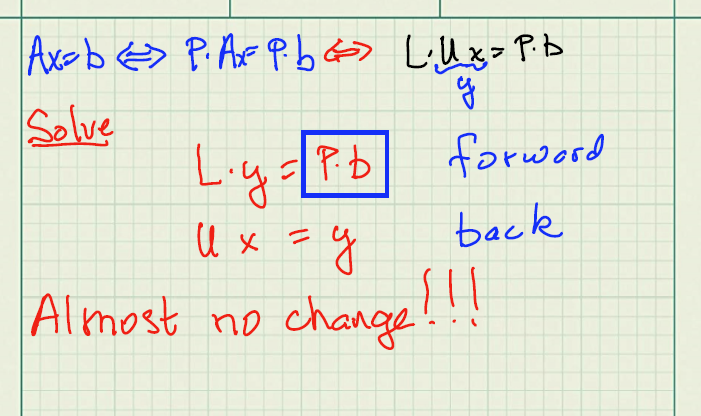
\includegraphics[width=0.9\columnwidth]{graphics/Summary/PeelingTheOnionPart04.png}

\end{center}

\begin{example}
\label{ex:SolveUsingLu01WithPerm} 
Use LU Factorization with permutations to solve the system of linear equations
\begin{equation}
    \label{eq:Chap5pt4AwithPerm}
\underbrace{\left[\begin{array}{rrr} -2 & -4 & -6\\
-2 & 1 & -4 \\ -2 & 11 & -4 \end{array}\right]}_{A}  \underbrace{\left[\begin{array}{r} x_1\\
x_2 \\ x_3\end{array}\right]}_{x} 
= \underbrace{\left[\begin{array}{r} 2\\
3 \\ -7 \end{array}\right]}_{b}. 
\end{equation}
\end{example}

\textbf{Solution:} This time we use the native LU function in Julia to compute $P \cdot A = L \cdot U$, with
\begin{equation}
    \label{eq:Chap5pt4LUwithPerm}
    \begin{aligned}
        P&= \left[
\begin{array}{ccc}
1.0 & 0.0 & 0.0 \\
0.0 & 0.0 & 1.0 \\
0.0 & 1.0 & 0.0 \\
\end{array}
\right]\\
L&= \left[ \begin{array}{ccc}
1.000 & 0.000 & 0.000 \\
1.000 & 1.000 & 0.000 \\
1.000 & 0.333 & 1.000 \\
\end{array}
\right]\\
U&= 
\left[
\begin{array}{rrr}
-2.000 & -4.000 & -6.000 \\
0.000 & 15.000 & 2.000 \\
0.000 & 0.000 & 1.333 \\
\end{array}
\right].
 \end{aligned}
\end{equation}
Even though $A$ admits an LU Factorization without row permutations, Julia inserts a permutation matrix. This is to improve the numerical accuracy on large problems. On our small problem, it's not really needed. Nevertheless, we'll use it to show that we obtain the same answer with essentially the same amount of work.\\

We first compute 
$$P b = \left[
\begin{array}{ccc}
1.0 & 0.0 & 0.0 \\
0.0 & 0.0 & 1.0 \\
0.0 & 1.0 & 0.0 \\
\end{array}
\right] \left[
\begin{array}{r}
2.0 \\
3.0 \\
-7.0 \\
\end{array}
\right] = \left[
\begin{array}{r}
2.0 \\
-7.0 \\
3.0 \\
\end{array}
\right]. $$
We then solve $L y = P b$ for the intermediate variable $y$, using forward substitution, 
$$\underbrace{\left[ \begin{array}{ccc}
1.000 & 0.000 & 0.000 \\
1.000 & 1.000 & 0.000 \\
1.000 & 0.333 & 1.000 \\
\end{array}
\right]}_{L} \underbrace{\begin{bmatrix}y_1 \\y_2 \\ y_3 \end{bmatrix}}_{y} =\underbrace{ \left[
\begin{array}{r}
2.0 \\
-7.0 \\
3.0 \\
\end{array}
\right]}_{P b} \implies\begin{bmatrix}y_1 \\y_2 \\ y_3 \end{bmatrix} = \left[
\begin{array}{r}
2.0 \\
-9.0 \\
4.0 \\
\end{array}
\right]. $$
And finally, we use this result to solve $U x = y$ for $x$, using back substitution,
$$ \underbrace{\left[
\begin{array}{rrr}
-2.000 & -4.000 & -6.000 \\
0.000 & 15.000 & 2.000 \\
0.000 & 0.000 & 1.333 \\
\end{array}
\right]}_{U} \underbrace{\begin{bmatrix}x_1 \\x_2 \\ x_3 \end{bmatrix}}_{x} =\underbrace{\left[
\begin{array}{r}
2.0 \\
-9.0 \\
4.0 \\
\end{array}
\right]}_{y} \implies\begin{bmatrix}x_1 \\x_2 \\ x_3 \end{bmatrix} = \left[
\begin{array}{r}
-8.0 \\
-1.0 \\
3.0 \\
\end{array}
\right]. $$
\Qed

\setcounter{chapter}{6}
\setcounter{section}{-1}
\section{A Grab Bag of Needed Results: Determinant of a Matrix Product, Matrix Inverses, Matrix Transpose, More on Permutation Matrices}

\begin{tcolorbox}
Let $A$ and $B$ be two $n \times n$ matrices. Then,
$$\det(A \cdot B) = \det(A) \cdot \det(B). $$
We note that $A$ and $B$ must be square and have the same size for the above useful fact to be true. 
\end{tcolorbox}

\vspace*{.2cm}
\begin{tcolorbox}[sharp corners, colback=green!30, colframe=green!80!blue, title=\textbf{\Large Matrix Determinant via LU Factorization}]
Now suppose that we have done the LU factorization of a square matrix $A$. Then, 
using the fact that the determinant of a product of two square matrices is the product their respective determinants, we have that 
$$\det(A) = \det(L \cdot U) = \det(L) \cdot \det(U). $$
Because $L$ and $U$ are triangular matrices, each of their determinants is given by the product of the diagonal elements. Hence, we have a way of computing the determinant for square matrices of arbitrary size.
\end{tcolorbox}

\vspace*{1cm}

{\bf \large Identity Matrix is Needed to Define the Matrix Inverse:} 
There is a special square matrix denoted $I$, or sometimes $I_n$ to emphasize that it is an $n \times n $ matrix, which has ones on its diagonal and zeros everywhere else,
$$I_1=[1],~I_2=\begin{bmatrix} 1 & 0\\0& 1 \end{bmatrix},~I_3= \begin{bmatrix} 1 & 0 & 0\\0& 1 & 0\\ 0 & 0 & 1 \end{bmatrix}, ~I_4=\begin{bmatrix} 1 & 0 & 0 & 0\\0& 1 & 0 & 0\\ 0 & 0 & 1 & 0 \\ 0 & 0& 0& 1\end{bmatrix}, ~\text{etc.} $$ 
Because $I_n$ is diagonal, we see immediately that $\det(I_n)=1$.

\begin{tcolorbox}[title=\textbf{\large Multiplication by the Identity Matrix}]
Suppose that $A$ is an $n \times m$ matrix. Then 
$$A = I_n \cdot A = A \cdot I_m. $$
In other words, as long as the matrix product is defined, multiplying a matrix (on either side) by an identity matrix does not change it. 
\end{tcolorbox}

\vspace*{1cm}

\begin{tcolorbox}[sharp corners, colback=green!30, colframe=green!80!blue, title=\textbf{\large The Inverse of a Square Matrix}]
 Let $A$ be an $n \times n$ matrix. A second $n \times n$ matrix $B$ is a multiplicative inverse of $A$ if
 $$A \cdot B = B \cdot A = I_n. $$
 \begin{itemize}
     \item When such a matrix exists, it can be shown to be unique.
     \item We say that $A$ is invertible and we denote the inverse by $A^{-1}$ and we simply call it $A$ inverse or the inverse of $A$.
     \item It is a major \textit{faux pas} (means, no-no, in French) to write $1/A$ in place of $A^{-1}$.
     \item \textbf{Very Useful Fact:} $A$ is invertible if, and only if, $\det(A) \neq 0$. It is so useful we will state it a second time below!
 \end{itemize}
\end{tcolorbox}
\vspace*{1cm}

\begin{tcolorbox}[sharp corners, colback=green!30, colframe=green!80!blue, title=\textbf{\large Most Important Matrix Inverse for ROB 101}]
 {\large Consider $A=\left[\begin{array}{rr} a & b \\ c & d\end{array} \right]$ and suppose that $\det(A) = a\cdot d - b \cdot c \neq 0.$ Then,
  $$ A^{-1}= \frac{1}{a\cdot d - b \cdot c} \left[\begin{array}{rr} d & -b \\ -c & a\end{array} \right] = \frac{1}{\det(A)} \left[\begin{array}{rr} d & -b \\ -c & a\end{array} \right] $$}
\end{tcolorbox}
\vspace*{1cm}

\textcolor{red}{\bf \large Key Facts About the Inverse:}
\begin{itemize}
    \item An $n \times n$ matrix $A$ is invertible if, and only if, $\det(A)\neq 0.$
    \item if $A$ and $B$ are both $n\times n$ and invertible, then their product is also invertible and
$$ \boxed{(A \cdot B)^{-1}=B^{-1} \cdot A^{-1}.} $$
Note that the order is swapped when you compute the inverse. To see why this is true, we note that
$$ (A\cdot B) \cdot (B^{-1} \cdot A^{-1}) =   A\cdot (B \cdot B^{-1})  \cdot A^{-1} = A\cdot (I)  \cdot A^{-1} = A\cdot A^{-1} = I.$$
\textbf{Hence, $(A\cdot B)^{-1} = B^{-1} \cdot A^{-1}$ and NOT $ A^{-1} \cdot B^{-1}$.}

\item Ax=b \iff x = A^{-1} \cdot b


\end{itemize}


\vspace*{1cm}

\begin{tcolorbox}[sharp corners, colback=lightergray, colframe=red, title=\textbf{\Large If at all Possible, Avoid Computing $A^{-1}$ Because it is Numerically Expensive}]
If what you really want to solve is $A x = b$, then it is numerically inefficient to first compute the matrix inverse, $A^{-1}$, and then to do the matrix multiplication $A^{-1} b$. This is because each column of $A^{-1}$ is the solution to a system of linear equations, namely,
\begin{equation}
\label{eq:SolveForInvA}
    A \cdot A^{-1} = I_n \iff A^{-1} = \left[\begin{array}{cccc} x^{\rm sol~1} & x^{\rm sol~2} & \cdots & x^{\rm sol~n}  \end{array} \right], \text{ where, }A x^{\rm sol~i} = e_i, 1 \le i \le n,
\end{equation}
and, in Julia notation, 
$$e_i[j]=\begin{cases} 1 &  \text{if}~~i = j \\ 0 & \text{otherwise}\end{cases}.$$
In other symbols, just to further drive home the point, solving for $A^{-1}$ is equivalent to solving $n$ different linear systems of equations, 
$$A x^{\rm sol~i} = e_i,$$ 
and then using the solutions as the columns of $A^{-1}$. 
%That is, 
% $$A^{-1} = \left[\begin{array}{cccc} x^{\rm sol~1} & x^{\rm sol~2} & \cdots & x^{\rm sol~n}  \end{array} \right]  \iff A x^{\rm sol~i} = e_i,~ 1 \le i \le n \iff A \cdot A^{-1} = I_n.$$
\end{tcolorbox}
\vspace*{1cm}

{\Huge Do you really want to solve $n$ systems of linear equations just to solve one? (That's a rhetorical question, and the answer is NO!)}\\ 

\begin{tcolorbox}[title=\textbf{\Large Transpose of a Matrix}]
Let $A$ be an $n \times m$ matrix with entries $[A]_{ij}=a_{ij}$. \\


$$
A^\top := \left[\begin{array}{c}\boxed{a_{11}~~ a_{12}~~ \cdots~~ a_{1m}} \medskip \\
\boxed{a_{21}~~ a_{22}~~ \cdots~~ a_{2m}} \\
\vdots \\
\boxed{a_{n1}~~ a_{n2}~~ \cdots~~ a_{nm}}\end{array}\right]^{\Huge \top} :=  \left[~~ \boxed{\begin{array}{c} a_{11} \\ a_{12}\\ \vdots \\ a_{1m}\end{array} }~~~
\boxed{\begin{array}{c} a_{21} \\ a_{22}\\ \vdots \\ a_{2m}\end{array} }~~~\cdots~~~
\boxed{\begin{array}{c} a_{n1} \\ a_{n2}\\ \vdots \\ a_{nm}\end{array}}~~\right].
$$
Equivalently, you can view the matrix transpose as taking each column of one matrix and laying the elements out as rows in the transposed matrix 
$$
 A^\top :=\left[ ~~\boxed{\begin{array}{c} a_{11} \\ a_{21}\\ \vdots \\ a_{n1}\end{array} }~~~
\boxed{\begin{array}{c} a_{12} \\ a_{22}\\ \vdots \\ a_{n2}\end{array} }~~~\cdots~~~
\boxed{\begin{array}{c} a_{1m} \\ a_{2m}\\ \vdots \\ a_{nm}\end{array} }~~\right]^{\Huge \top}:=  \left[\begin{array}{c}\boxed{a_{11}~~ a_{21}~~ \cdots~~ a_{n1}} \medskip \\
\boxed{a_{12}~~ a_{22}~~ \cdots~~ a_{n2}} \\
\vdots \\
\boxed{a_{1m}~~ a_{2m}~~ \cdots~~ a_{nm}}\end{array}\right] .
$$
\end{tcolorbox} 

\begin{tcolorbox}[title=\textbf{\Large Properties of the Transpose Operation}]
For any matrix $A$, 
$$(A^\top)^\top = A \text{  and if }A \text{ is square }, \det(A^\top) = \det(A). $$
Suppose that $A$ is $n \times m$ and $B$ is $m \times p$, so that $A \cdot B$ makes sense. Then
$$ (A \cdot B)^\top = B^\top \cdot A^\top, $$
\textbf{and just as with the matrix inverse, the order of the matrices is reversed.}  \end{tcolorbox}

\begin{tcolorbox}[[sharp corners, colback=lightergray, colframe=red, title=\textbf{\Large  Symmetric and Skew-symmetric Matrices}] \Large 
An $n \times n$ matrix is \textbf{symmetric} if $A^\top = A$ (the transpose of $A$ is equal to $A$ itself). An $n \times n$ matrix is \textbf{skew-symmetric} if $A^\top = -A$ (the transpose of $A$ is equal to minus $A$). 
\end{tcolorbox}
\vspace*{0.2cm}

\begin{example}
Determine which matrices are symmetric, skew-symmetric, or neither.
$$
A_1=\left[
\begin{array}{rrr}
1 & -2 & 5\\
2 & 0 & 6\\
-5 & -6 & 7
\end{array} \right],~~A_2=\left[
\begin{array}{rrr}
1 & 3 & 7\\
3 & 0 & -6\\
7 & -6 & 7
\end{array} \right],~~
A_3=\left[
\begin{array}{ccc}
1 & 2 & 3\\
4 & 5 & 6
\end{array} \right], ~\text{and}~A_4=\left[
\begin{array}{rrr}
0& -2 & 5\\
2 & 0 & 6\\
-5 & -6 & 0
\end{array} \right].
$$
\end{example}

\noindent \textbf{Solution:}
We compute each of the transposes and then compare them to either the original matrix or its negative, to check for the matrix being symmetric, skew-symmetric, or neither.
$$
A_1^\top=\left[
\begin{array}{rrr}
1 & 2 & -5\\
-2 & 0 & -6\\
5 & 6 & 7
\end{array} \right],~~A_2^\top=\left[
\begin{array}{rrr}
1 & 3 & 7\\
3 & 0 & -6\\
7 & -6 & 7
\end{array} \right],~~
A_3^\top=\left[
\begin{array}{cc}
1 & 4 \\
2 & 5 \\
3 & 6
\end{array} \right], ~\text{and}~A_4^\top=\left[
\begin{array}{rrr}
0& 2 & -5\\
-2 & 0 & -6\\
5 & 6 & 0
\end{array} \right].
$$
Because $A_1^\top$ is neither equal to $A_1$ nor $-A_1$, it is neither symmetric nor skew-symmetric. Because $A_2^\top$ equals $A_2$ it is symmetric. Because $A_3$ is not square, it cannot be either symmetric or skew-symmetric. Because $A_4^\top$ equals $-A_4$, it is skew-symmetric.
\Qed

\setcounter{chapter}{7}
\setcounter{section}{-1}
\section{The Vector Space $\real^n$: Part 1}

{\large 
\section*{Learning Objectives}
\begin{itemize}
\item Instead of working with individual vectors, we will work with a collection of vectors. 
\item Our first encounter with some of the essential concepts in Linear Algebra that go beyond systems of equations.
\end{itemize}

\section*{Outcomes}
\begin{itemize}
\item Vectors as $n$-tuples of real numbers
\item $\real^n$ as the collection of all $n$-tuples of real numbers
\item Linear combinations of vectors
\item Linear independence of vectors
\item Relation of these concepts to the existence and uniqueness of solutions to $Ax=b$.
\item How the LU Factorization makes it very straightforward to check the linear independence of a set of vectors, and how a small modification to the LU factorization makes it equally straightforward to check if one vector is a linear combination of a set of vectors. 
\end{itemize}
}

\section{Vectors in $\real^n$ }
An $n$-tuple is a fancy name for an ordered list of $n$ numbers, $(x_1, x_2, \ldots, x_n)$. If this sounds a lot like a vector, then good, because \textbf{we will systematically identify}
\begin{equation}
\real^n:=\{(x_1, x_2, \ldots, x_n)~|~x_i \in \real, 1\le i \le n \} 
\end{equation}
\textbf{with column vectors}. In other words, for us,
\begin{equation}
\real^n:=\{(x_1, x_2, \ldots, x_n)~|~x_i \in \real, 1\le i \le n \} \iff \left\{\begin{bmatrix} x_1 \\ x_2 \\ \vdots \\ x_n\end{bmatrix} ~\Bigg|~  x_i \in \real, 1\le i \le n \right\}=:\real^n.
\end{equation}
The choice of identifying $n$-tuples of numbers with column vectors instead of row vectors is completely arbitrary, and yet, it is very common.

\begin{tcolorbox}[sharp corners, colback=green!30, colframe=green!80!blue,
title=\textbf{\Large Columns of Matrices are Vectors and Vice Versa}]
Suppose that $A$ is an $n\times m$ matrix, then its columns are vectors in $\real^n$ and conversely, given vectors in $\real^n$, we can stack them together and form a matrix:
\begin{equation}
\label{eq:ColumnsOfMatrixVectorsRn}
    A =  \left[\begin{array}{cccc} a_{11}& a_{12}& \cdots & a_{1m} \\
 a_{21}& a_{22}& \cdots & a_{2m}  \\
 \vdots & \vdots&  \ddots & \vdots \\
 a_{n1}& a_{n2}& \cdots & a_{nm} 
 \end{array}\right] =
\left[\begin{array}{cccc} a_1^{\rm col} & a_2^{\rm col} & \cdots & a_m^{\rm col}\end{array}\right]  \iff a_j^{\rm col}:=\begin{bmatrix} a_{1j} \\ a_{2j}  \\ \vdots \\ a_{nj} \end{bmatrix} \in \real^n, 1 \le j \le m
\end{equation}
\end{tcolorbox}


\section{Linear Combinations of the Columns of a Matrix A}


\begin{tcolorbox}[sharp corners, colback=green!30, colframe=green!80!blue,title=\textbf{Linear Combination of the Columns of A}]
\textbf{Definition} The following sum of scalars times vectors,
\begin{equation}
    \label{eq:EarlyDefLinearCombination}
    \alpha_1 \begin{bmatrix} a_{11} \\ a_{21}\\ \vdots \\ a_{n1} \end{bmatrix}  + \alpha_2  \begin{bmatrix} a_{12} \\ a_{22}\\ \vdots \\ a_{n2} \end{bmatrix}  + \cdots + \alpha_m \begin{bmatrix} a_{1m} \\ a_{2m}\\ \vdots \\ a_{nm} \end{bmatrix},
\end{equation}
is called a \textbf{linear combination} of the columns of $A$. When we set $A\alpha = b$, and turn it around as $b =A \alpha$, we arrive at an important \textbf{Fact:} a vector $\alpha \in \real^m$ is a solution to $Ax=b$ (that is, $A \alpha = b$) if, and only if
\begin{equation}
    \label{eq:EarlyDefLinearCombinationWithb}
   b= \alpha_1 \begin{bmatrix} a_{11} \\ a_{21}\\ \vdots \\ a_{n1} \end{bmatrix}  + \alpha_2  \begin{bmatrix} a_{12} \\ a_{22}\\ \vdots \\ a_{n2} \end{bmatrix}  + \cdots + \alpha_m \begin{bmatrix} a_{1m} \\ a_{2m}\\ \vdots \\ a_{nm} \end{bmatrix},
\end{equation}
that is, $b$ can be expressed as a linear combination of the columns of $A$.
We will revisit this later, but \eqref{eq:EarlyDefLinearCombinationWithb} is a primary motivation for introducing the notion of linear combinations.
\end{tcolorbox}

\section{Linear Combinations of Vectors in $\real^n$}

\begin{tcolorbox}[title=\textbf{Linear Combination}]
A vector $v\in \real^n$ is a \textbf{linear combination of} $\{u_1, u_2, \ldots, u_m\} \subset \real^n$ if there exist real numbers $\alpha_1, \alpha_2, \ldots, \alpha_m$ such that
\begin{equation}
    \label{eq:DefLinearCombinationRn}
    v = \alpha_1 u_1 + \alpha_2 u_2 + \cdots + \alpha_m u_m.
\end{equation}

\end{tcolorbox}

\section{Existence of Solutions to Ax=b}
\label{sec:UniquenessSolutions}

Let $A$ be an $n \times m$ matrix, not necessarily square, as in \eqref{eq:ColumnsOfMatrixVectorsRn}. Recall that columns of $A$ and vectors in $\real^n$ are the same thing. We write out $Ax=b$ is all its glory, 
\begin{equation}
\label{eq:ExistenceSolutionsNonsquare}    
 \underbrace{\left[\begin{array}{cccc} a_{11}& a_{12}& \cdots & a_{1m} \\
 a_{21}& a_{22}& \cdots & a_{2m}  \\
 \vdots & \vdots&  \ddots & \vdots \\
 a_{n1}& a_{n2}& \cdots & a_{nm} 
 \end{array}\right] }_{A} \underbrace{\left[ \begin{array}{c} x_1 \\ x_2 \\
\vdots \\ x_m   \end{array} \right]}_{x} = \underbrace{\left[ \begin{array}{c} b_1 \\ b_2 \\ \vdots \\ b_n  \end{array} \right]}_{b}.
\end{equation}

\vspace*{.5cm}
\begin{tcolorbox}[sharp corners, colback=green!30, colframe=green!80!blue, title=\textbf{\large Existence of Solutions}] 
The equation $Ax=b$ has a solution if, and only if, $b$ can be written as a linear combination of the columns of $A$.
\end{tcolorbox}

\textbf{The following is more or less a proof:} Suppose that $\bar{x}$ satisfies $A \bar{x} =b$, which is the same thing as saying $\bar{x}$ is a solution of $Ax=b$. Then, doing the indicated multiplication of $A \bar{x}$ via our now favorite method, the columns of $A$ times the rows of the vector $\bar{x}$, which are its scalar entries $\bar{x}_i$, yields
\begin{equation}
    \label{eq:bIsLinearCombinationColumnsA02}
\begin{bmatrix} a_{11} \\ a_{21}\\ \vdots \\ a_{n1} \end{bmatrix} \bar{x}_1 +  \begin{bmatrix} a_{12} \\ a_{22}\\ \vdots \\ a_{n2} \end{bmatrix} \bar{x}_2 + \cdots + \begin{bmatrix} a_{1m} \\ a_{2m}\\ \vdots \\ a_{nm} \end{bmatrix} \bar{x}_m = \begin{bmatrix} b_1 \\ b_2\\ \vdots \\ b_m \end{bmatrix}
\end{equation}
Exchanging the two sides of the equal sign and moving the scalars $\bar{x}_i$ to the front of the vectors give
\begin{equation}
    \label{eq:bIsLinearCombinationColumnsAflipped}
 \begin{bmatrix} b_1 \\ b_2\\ \vdots \\ b_m \end{bmatrix} = \bar{x}_1 \begin{bmatrix} a_{11} \\ a_{21}\\ \vdots \\ a_{n1} \end{bmatrix}+ \bar{x}_2 \begin{bmatrix} a_{12} \\ a_{22}\\ \vdots \\ a_{n2} \end{bmatrix} + \cdots + \bar{x}_m \begin{bmatrix} a_{1m} \\ a_{2m}\\ \vdots \\ a_{nm} \end{bmatrix};
\end{equation}
in other words, $b$ is a linear combination of the columns of $A$. The other way around works as well: if we manage to write 
$$b = c_1  a_1^{\rm col} + c_2 a_2^{\rm col} + \cdots c_m a_m^{\rm col}$$
for some real numbers $c_i \in \real$, then $\bar{x}=\begin{bmatrix} c_1 & c_2 & \cdots & c_m \end{bmatrix}^\top$ satisfies $A \bar{x}=b$, and hence it is a solution to $Ax=b$. \\

Recall that $a_j^{\rm col}:=\begin{bmatrix} a_{ij} & a_{2j}  & \cdots & a_{nj} \end{bmatrix}^\top, 1 \le j \le m.$


\section{Linear Independence in $\real^n$}

The definition of linear independence of an ``abstract'' set of vectors in $\real^n$ is 100\% motivated by the study of the uniqueness of solutions to $Ax=0.$ Of course, vectors in $\real^n$ are columns of $n \times m$ matrices, so who's to say what is abstract and what is not!

\vspace*{0.5cm}

\begin{tcolorbox}[sharp corners, colback=green!30, colframe=green!80!blue, title=\textbf{Linear Independence of a Set of Vectors}]
 The set of vectors $\{v_1, v_2, ..., v_m \} \subset \real^n$ is \textbf{linearly dependent} if there exist real numbers $\alpha_1, \alpha_2, \ldots, \alpha_m$ \textbf{NOT ALL ZERO} yielding a linear combination of vectors that adds up to the zero vector,
\begin{equation}
    \alpha_1 v_1 + \alpha_2 v_2 + \ldots + \alpha_m v_m =0_{n \times 1}.
\end{equation}

On the other hand, the vectors $\{v_1, v_2, ..., v_m \}$ are \textbf{linearly independent} if the \textbf{only} real numbers $\alpha_1, \alpha_2, \ldots, \alpha_m$ yielding a linear combination of vectors that adds up to the zero vector,
\begin{equation}
    \alpha_1 v_1 + \alpha_2 v_2 + \ldots + \alpha_m v_m =0_{n \times 1},
    \end{equation}
are $\boldsymbol{\alpha}_1= \mathbf{0}, \boldsymbol{\alpha}_2=\mathbf{0}, \ldots, \boldsymbol{\alpha}_m=\mathbf{0}.$\\

\textbf{Concise Definition of Linear Independence:} 
$$\alpha_1 v_1 + \alpha_2 v_2 + \ldots + \alpha_m v_m =0_{n \times 1}  \iff \begin{bmatrix} \alpha_1 \\ \alpha_2 \\ \vdots \\ \alpha_m \end{bmatrix} = \begin{bmatrix} 0 \\ 0 \\ \vdots \\ 0 \end{bmatrix}= 0_{m \times 1}.$$
\end{tcolorbox}

\begin{tcolorbox}[[sharp corners, colback=lightergray, colframe=red, title=\textbf{\Large  Remark on Sets of Linearly Dependent Vectors}] \Large 

\begin{itemize}
    \item A set consisting of one n-vector $\{v_1 \}$ is linearly \textbf{dependent} if, and only if, $v_1 = 0_{n \times 1}$. 

    \item A set consisting of $m>1$ vectors $\{v_1, v_2, \ldots, v_m \}$ is linearly \textbf{dependent} if, and only if, one of the vectors in the set can be written as a linear combination of other vectors in the set.    
    
\end{itemize}
\end{tcolorbox}
\vspace*{0.2cm}
\textbf{The following is a proof of the second statement.} Suppose $\{v_1, v_2, \ldots, v_m \}$ is linearly \textbf{dependent}. Then there exist $\alpha_1$ to $\alpha_m$ NOT ALL ZERO such that 
$$ \alpha_1 v_1 + \alpha_2 v_2 + \cdots + \alpha_m v_m = 0_{n \times 1}.$$
Let $\alpha_k$ be the first non-zero coefficient among $\alpha_1$ to $\alpha_m$. Then 
$$ \alpha_k v_k + \alpha_{k+1} v_{k+1} + \cdots + \alpha_m v_m = 0_{n \times 1},$$
because $\alpha_k$ being the first non-zero coefficient means that $\alpha_1 = \cdots = \alpha_{k-1}=0$. 
Because $\alpha_k \neq 0$, we can write
\begin{align*} 
\alpha_k v_k & = -\alpha_{k+1} v_{k+1} - \cdots - \alpha_m v_m \\
& \Updownarrow \\
v_k & = - \frac{\alpha_{k+1}}{\alpha_k} v_{k+1} - \cdots - \frac{\alpha_{m}}{\alpha_k}v_m 
\end{align*}
which shows that we can write $v_k$ as a linear combination of other vectors in the set.\\

For the other direction, suppose that for some $k$, $v_k$ can be written as a linear combination of other vectors in the set, namely
$$ v_k = \sum_{i \neq k} \beta_i v_i.$$
Then, 
$$ \sum_{i \neq k} \beta_i v_i -v_k = 0_{n \times 1} $$
and thus we have
$$ \alpha_1 v_1 + \alpha_2 v_2 + \cdots + \alpha_m v_m = 0_{n \times 1},$$
with 
$$ \alpha_i = \begin{cases}
    -1 \neq 0 & i = k \\
    \beta_i & i \neq k
\end{cases}
 $$
 and thus the set is linearly dependent; we have a linear combination that sums up to the zero vector with at least one coefficient that is non-zero. \Qed \\

 \section{Existence and Uniqueness of Solution to $Ax = b$, without assuming $A$ is Square}
\begin{tcolorbox}[sharp corners, colback=green!30, colframe=green!80!blue, title=\textbf{\large Existence and Uniqueness of Solutions to $Ax=b$}]
The following two statements are equivalent
\begin{enumerate}
\renewcommand{\labelenumi}{(\alph{enumi})}
\setlength{\itemsep}{.2cm}
\item The system of linear equations $Ax=b$ has a solution, and, it is unique.

\item $b$ is a linear combination of the columns of $A$, and, the columns of $A$ are linearly independent. 
\end{enumerate}

\textbf{Remark:} If $b$ is not a linear combination of the columns of $A$, then $Ax=b$ does not have a solution. If the columns of $A$ are not linearly independent, then if $Ax=b$ has one solution, it also has an infinite number of solutions. \\


\end{tcolorbox}

\vspace*{.5cm}



\section{A Pro Tip for Checking Linear Independence}
\label{sec:proTipLinearIndependence}

\begin{tcolorbox}[sharp corners, colback=green!30, colframe=green!80!blue,
title=\textbf{Pro-tip! Linear Independence in a Nutshell}]
Consider the vectors in $\real^n$,
$$\left\{v_1=\begin{bmatrix} a_{11} \\ a_{21}\\ \vdots \\ a_{n1} \end{bmatrix},  v_2=\begin{bmatrix} a_{12} \\ a_{22}\\ \vdots \\ a_{n2} \end{bmatrix}, ...,  v_m=\begin{bmatrix} a_{1m} \\ a_{2m}\\ \vdots \\ a_{nm} \end{bmatrix} \right\},$$ 
and use them as the columns of a matrix that we call $A$,
\begin{equation}
\label{eq:MatrixFromLinearIndependence_proTipC}    
A=\left[\begin{array}{cccc} a_{11}& a_{12}& \cdots & a_{1m} \\
 a_{21}& a_{22}& \addsts & a_{2m}  \\
 \vdots & \vdots&  \ddots & \vdots \\
 a_{n1}& a_{n2}& \cdots & a_{nm} 
 \end{array}\right].
 \end{equation}
 The following statements are equivalent:
 \begin{itemize}
     \item  The set of vectors $ \{v_1, v_2, \ldots, v_m \} $ is linearly independent.
     \item The $m \times m$ matrix $A^\top \cdot A$ is invertible. 
     \item $\det(A^\top \cdot A) \neq 0$.
     \item For any LU Factorization $P \cdot (A^\top \cdot A) = L \cdot U$  of $A^\top A$, the $m \times m$ upper triangular matrix $U$ has no zeros on its diagonal.
 \end{itemize}
 \end{tcolorbox}

\vspace*{.3cm}


\section{Uber Pro Tip for Counting the Number of Linearly Independent Vectors in a Set}

\begin{tcolorbox}[sharp corners, colback=green!30, colframe=green!80!blue,
title=\textbf{ {\Large \textcolor{red}{\bf Uber} Pro-Tip:} \large Number of Linearly Independent Vectors via an Enhanced LU Factorization}]
Assume that a set of vectors has been stacked to form the columns of an $n \times m$ matrix $A$ , or that the matrix $A$ has been given to us directly. \textbf{Fact:} The matrix $A^\top \cdot A$ always has an \textbf{LDLT Factorization}
\begin{equation}
    \label{eq:LDLTfactorization}
    P\cdot A^\top \cdot A \cdot P^\top = L\cdot D \cdot L^\top,
\end{equation}
where
\begin{itemize}
    \item $P$ is a (row) permutation matrix;
    \item $P^\top$, the transpose of $P$, permutes the columns of $A$;
    \item $L$ is uni-lower triangular and $L^\top$, the transpose of $L$, is therefore uni-upper triangular; and
    \item $D$ is diagonal and has non-negative entries.
\end{itemize}
\textcolor{red}{\bf Moreover,}
\begin{itemize}
    \item \textcolor{red}{\bf the number of linearly independent columns of $A$ is equal to the number of non-zero entries on the diagonal of $D$;} and, if we denote this number by $k$,
    \item  \textcolor{red}{\bf for the version of the LDLT given in our textbook, the first $k$-columns of $A \cdot P^\top$ are linearly independent, and the remaining $(m-k)$-columns (if any) are linearly dependent on the first $k$ columns.} 
    \item Because the columns of $A\cdot P^\top$ are simply the columns of $A$ permuted by $P^\top$ (that is, re-ordered by the permutation matrix), \textcolor{red}{\bf the first $k$-columns of $A \cdot P^\top$ provide a selection of linearly independent columns of $A$}.
\end{itemize}

\end{tcolorbox}

\vspace*{.2cm} 
\textbf{Remarks:}The LDLT factorization may look intimidating, but once you realize that $U:=D \cdot L^\top$ is upper triangular, this is really a refined LU Factorization that is possible for matrices of the form $A^\top \cdot A$. The name \textcolor{blue}{\bf LDLT Factorization} comes from $L\cdot D \cdot L^\top$, where the last \textcolor{blue}{\bf T} stands for transpose. It is also called a \textbf{Cholesky Factorization}. Whatever you call it, it is simply our well-known LU Factorization with $U$ in the special form  $U:=D \cdot L^\top$, which is possible for special kinds of matrices of the form $A^\top \cdot A$. \\

\section{Attractive Test for Linear Combinations}
\label{sec:AttractiveTestLinearCombination}

\begin{tcolorbox}[sharp corners, colback=green!30, colframe=green!80!blue,
title=\textbf{Pro Tip! Linear Combination or Not?}]
\textbf{Fact:} A vector $v_0\in \real^n$ can be written as a linear combination of $\{v_1, \ldots, v_m\} \subset \real^n$  if, and only if, the set $\{v_0, v_1, \ldots, v_m\}$ has the same number of linearly independent vectors as $\{v_1, \ldots, v_m\}$.\\

Applying this to determining if a linear system of equations $Ax=b$ has a solution, we first define $A_{\rm e} :=\left[A~~ b \right]$ by appending $b$ to the columns of $A$. Then we do the corresponding LDLT Factorizations
\begin{itemize}
    \item $P \cdot \left(A^\top \cdot A \right)\cdot P^\top = L \cdot D \cdot L^\top$
    \item $P_{\rm e} \cdot \left(A_{\rm e}^\top \cdot A_{\rm e}  \right) \cdot P^\top_{\rm e} = L_{\rm e} \cdot D_{\rm e} \cdot L^\top_{\rm e} $.
\end{itemize}

\textbf{Fact:}  $Ax=b$ has a solution if, and only if, $D$ and $D_{\rm e}$ have the same number of non-zero entries on their diagonals.\\

Why? We know that $Ax=b$ has a solution if, and only if, $b$ is a linear combination of the columns of $A$. That is, $A$ and $A_e:=[A~~b]$ must have the same number of linearly independent columns.\\

\textbf{(Optional Remark):} You get the same result by defining $A_{\rm e} :=\left[b~~ A \right]$; in fact, you can insert $b$ anywhere you want, even in the middle of the columns of $A$.
\end{tcolorbox}

\vspace*{.5cm}
\end{document}